\documentclass[UTF8]{ctexart}
\hfuzz=4pt

\usepackage{parskip}
    \setlength{\parindent}{0em}
    \setlength{\parskip}{1em}
\usepackage{geometry}
    \geometry{left=4cm,right=4cm,top=2cm,bottom=2cm}
\usepackage{amsmath, amssymb, amsthm, mathtools}
\usepackage{thmtools}
    \renewcommand\qedsymbol{$\blacksquare$}
    \declaretheorem[numberwithin=section,shaded={rulecolor=cyan,rulewidth=2pt,bgcolor=white}]{definition}
    \declaretheorem[numberwithin=section,shaded={rulecolor=orange,rulewidth=2pt, bgcolor=white}]{theorem}
    \newtheoremstyle{mystyle}{1em plus .2 em minus .2em}{1em plus .2 em minus .2em}{}{}{\bfseries}{.}{.5em}{}
    \theoremstyle{mystyle}
    \newtheorem{axiom}{Axiom}[section]
    \newtheorem{lemma}{Lemma}[section]
    \newtheorem{proposition}{Proposition}[section]
    \newtheoremstyle{myremark}{1em plus .2 em minus .2em}{1em plus .2 em minus .2em}{}{}{\itshape}{.}{.5em}{}
    \theoremstyle{myremark}
    \newtheorem*{remark}{Remark}
    \theoremstyle{plain}
    \newtheorem{corollary}{Corollary}[section]
    \newenvironment{explanation}{\textit{说明}.}{\hfill$\blacksquare$}
\usepackage{caption}
\usepackage{xcolor}
\usepackage{graphicx}
\usepackage{float}
\usepackage{setspace} 	 % 行间距 \begin{spacing}{arg}
\usepackage{esint}
\usepackage{hyperref}
    \hypersetup{colorlinks=true,linktoc=all,linkcolor=blue}

\newcommand{\ve}[1]{\boldsymbol{\mathbf{#1}}}
\newcommand{\unit}[1]{\boldsymbol{\mathbf{\hat{#1}}}}
\renewcommand{\r}{\mathrm}
\renewcommand{\cal}{\mathcal}
\newcommand{\scr}{\mathscr}

\newcommand{\E}{\mathrm e}
\renewcommand{\I}{\mathrm i}
\newcommand{\R}{\mathbb R}
\newcommand{\Z}{\mathbb Z}
\newcommand{\N}{\mathbb N}
\newcommand{\Q}{\mathbb Q}
\renewcommand{\C}{\mathbb C}
\DeclarePairedDelimiter\set{\{}{\}}
\newcommand{\connect}[1][]{\mathrel{\overset{#1}{\mbox{---}}}}

\pagestyle{empty}

\begin{document}
\section{图与子图}
下面概念描述了由原图得到其它图的方法.
\begin{definition}[\text{子图}]
    设图 $ G = (V, E) $, $ V' \subseteq V $, $ E' \subseteq E $, 则图 $ G' = (V', E') $ 称为 $ G $ 的子图. 若 $ G' \neq G $, 则称 $ G' $ 为 $ G $ 的真子图.
\end{definition}

相比子图, 导出子图的概念更常见.

\begin{definition}[\text{点导出子图}]
    设 $ G = (V, E) $, $ V' \subseteq V $. 定义 $ V' $ 的点导出子图 (vertex-induced subgraph) 为 $ G(V') = (V', E') $, 其中:
    \[ E' \coloneqq \set{(a, b) \in E \mid a, b \in V'} \,.\]
\end{definition}

换句话说, $ G(V') $ 的边集由 $ E $ 中关联 $ V' $ 中任意顶点的的边构成. 这意味着两方面: (1) $ V' $ 中任意两点若在 $ G $ 中关联, 则这条边就在导出子图中; (2) 若 $ (a, b) $ 为导出子图中的一条边, 则 $ a, b $ 在原图中也是关联的.

同理还可得到边导出子图: 设图 $ G $ 边集的子集 $ E' \subseteq E(G) $, 则 $ E' $ 的边导出子集:
\[ \begin{cases}
    V(G(E')) \coloneqq \set{a \mid \exists b, (a, b) \in E'} \\
    E(G(E')) = E'
\end{cases} \,.\]

\begin{definition}[\text{删除点}]
    对于图 $ G = (V, E) $, 设 $ v \in V $. 则删掉这个点及其关联的边, 剩下的图记作 $ G - v $. 也即:
    \[ \begin{cases}
        V(G - v) \coloneqq V - \set{v} \\
        E(G - v) \coloneqq \set{(a, b) \in E \mid a \neq v \land b \neq v} 
    \end{cases} \,.\]

    注意: $ E(G - v) $ 的等价定义为 $ \set{(a, b) \in E \mid a, b \in V - \set{v}} $.
    \vskip 1em
    同理还可以得到删除多个点及其中每个点关联的边得到的图, 记点集 $ V' \subseteq V $. 则 $ G - V' $ 可以定义为:
    \[ \begin{cases}
        V(G - V') \coloneqq V - V' \\
        E(G - V') \coloneqq \set{(a, b) \in E \mid a, b \in V - V'} 
    \end{cases} \,.\]
\end{definition}

从导出子图以及删点子图的定义, 不难得到下面的结论:
\begin{proposition}
    设 $ G = (V, E) $, 若 $ V' $ 和 $ V'' $ 为 $ V $ 的一个划分, 即: $ V' \cap V'' = \varnothing $ 且 $ V' \cup V'' = V $. 则有:
    \[ G(V') = V - V'' \,,\]
    \[ G(V'') = V - V' \,.\]
\end{proposition}

也就是说, 导出子图 $ G(V') $ 可以定义为删去所有除 $ V' $ 之外的点 (即 $ V'' $) 以及其关联的边后剩下的图.

\subsection{点度}
\begin{definition}[\text{度}]
    无向图中, 点 $ v $ 的度数定义为与这个点相关联的边的数目, 记作 $ d(v) $ 或 $ \deg(v) $. 有向图中, 点 $ v $ 的度分为出度和入度: 出度为以 $ v $ 为起点的边的数目, 记作 $ d^+(v) $; 入度为以 $ v $ 为终点的边的数目, 记作 $ d^-(v) $.
\end{definition}

\begin{remark}
    出度为正, 入度为负的规定方式和散度的正负类似.
\end{remark}

图 $ G $ 中, 最大点度和最小点度定义为:
\[ \Delta \coloneqq \max \set{d(v) \mid v \in V(G)} \,,\]
\[ \delta \coloneqq \min \set{d(v) \mid v \in V(G)} \,.\]

\begin{theorem}[\text{握手定理}]
    无向图 $ G = (V, E) $ 满足所有点度之和等于边数量的两倍:
    \[ \sum_{v \in V} d (v) = 2 |E| = 2 \varepsilon(G) \,.\]

    而在有向图中, 有类似的关系:
    \[ \sum_{v \in V} d^+(v) = \sum_{v \in V} d^-(v) =  \varepsilon(G) \,.\]
\end{theorem}

由握手定理可以得到下面的推论 (为引述方便, 称度数为奇数的点为奇点, 度数为偶数的点为偶点):
\begin{proposition}
    对于任意简单无向图, 奇点的个数一定为偶数.
\end{proposition}



\section{无向图的连通性}
\begin{definition}[\text{道路, 简单道路与路径}]
    定义道路 (walk) 为一系列交替的点和边的序列: $ v_0, e_1, v_1, e_2, v_2, \dots, e_n, v_n $; 其中 $ e_i $ 关联 $ v_{i - 1} $ 和 $ v_i $. 
    \begin{itemize}
        \item 若道路中除首尾两个点, 没有相同的节点, 即对任意 $ 1 \leqslant i, j \leqslant n - 1 $, 有 $ v_i \neq v_j $, 则称该道路为简单道路 (path)
        \item 若道路中没有重复的边, 则称其为路径 (trail)
        \item 若道路首尾两点为同一点, 则称其为回路; 若简单道路的首位两点为同一点, 则称其为简单回路
    \end{itemize}
\end{definition}

\begin{remark}
    可以看出, 从道路, 到路径, 到简单道路, 条件逐渐加强. 
\end{remark}

\begin{table}[H]
    \centering
    \begin{tabular}{c|ccc|cc}
        限制 & 英文 & 翻译1 & 翻译2 & 闭合时 & 闭合时翻译 \\ \hline
            & walk & 道路 & 道路 & closed walk & 回路 \\ \hline
        edge-distinct & trail & 简单道路 & 路径 & circuit & 简单回路 \\ \hline
        vertex-distinct & path & 基本道路 & 简单道路 & cycle & 环/圈(基本回路)
    \end{tabular}
\end{table}

对于道路 $ v_0, e_1, v_1, \dots, v_{n - 1}, e_n, v_n $, 其含有 $ n $ 条边, 称这条道路的长度为 $ n $, 记作 $ d(v_0, v_n) = n $.

下面几张示意图描述了上面几个术语之间的区别, 注意箭头并不表示有向图, 数字也不代表赋权, 此处只是形象化的表示出这条道路从起点到终点的行进过程和顺序.
\begin{figure}[H]
    \centering
    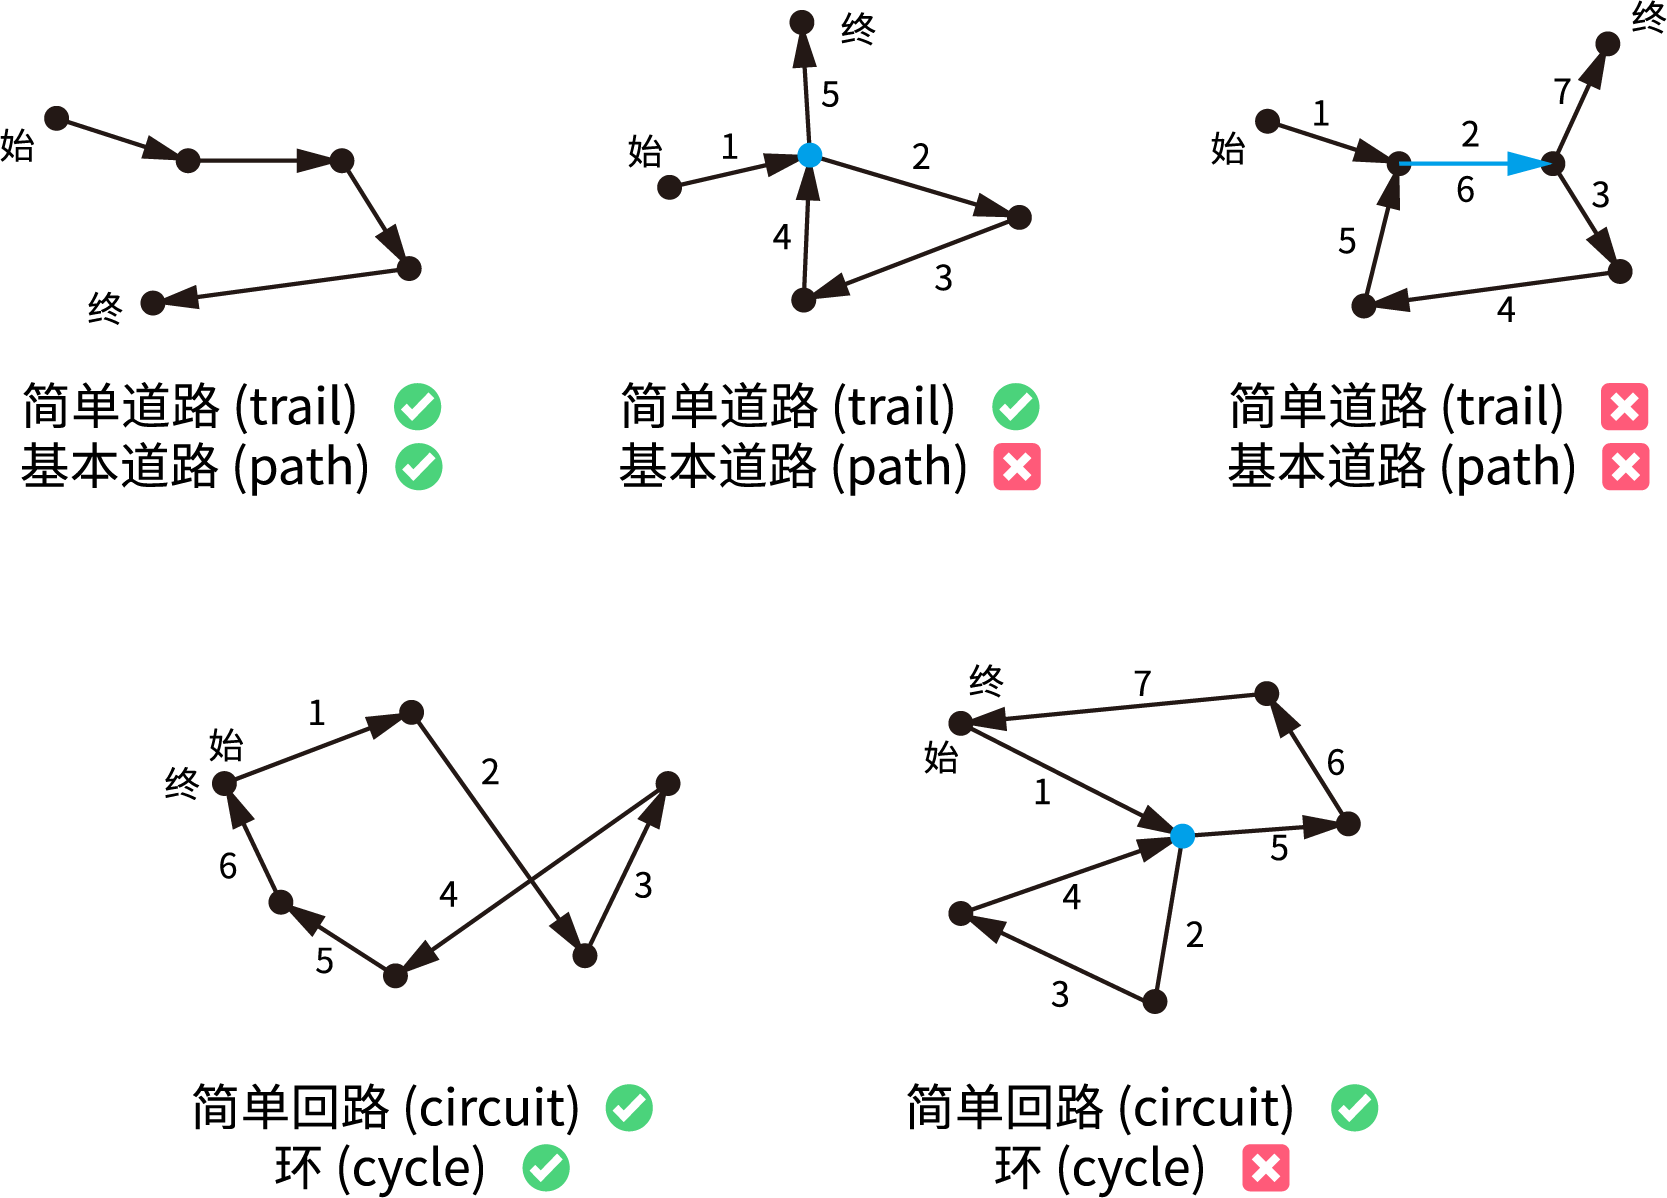
\includegraphics[width = 0.9\linewidth]{./images/walks.png}
\end{figure}


\begin{lemma}
    简单图中, 任何简单回路都包含圈. (任何简单图都可分为多个圈 ?)
\end{lemma}

\begin{explanation}
    如果简单回路中不存在重复内点, 则其自身就是圈.

    如果简单回路不是圈, 则其存在重复的内点 $ v_i = v_j $. 删掉其中的回路, 得到 $ v_0, e_1, v_1, \dots v_i, e_{j + 1}, v_{j + 1}, \dots, v_{n} = v_0 $, 如果剩下的回路不是圈, 则重复上面的步骤, 最终能够得到一个圈. 
\end{explanation}

\begin{lemma}
    边 $ e $ 在圈中 $ \iff $ $ e $ 在简单回路中.
\end{lemma}

\begin{proof}
    设 $ e $ 在圈中, 由于一个圈必然是一个简单回路, 所以 $ e $ 也在简单回路中.

    设边 $ e $ 为简单回路 $ v_0, e_1, v_1, \dots, e_n, v_n $ 的一条边, 任何简单回路都可以由几个圈组成, 故 $ e $ 也在其中.
\end{proof}



\begin{definition}[\text{连通}]
    对于无向图 $ G $ 中的两点 $ a $, $ b $, 称这两点是连通的, 如果能够找到一条道路, 使得 $ a $ 为起点 $ b $ 为终点或 $ b $ 为起点 $ a $ 为终点. 称 $ G $ 是连通的, 当且仅当任意 $ u, v \in V(G) $, $ u $ 和 $ v $ 是连通的.
\end{definition}

\paragraph{例}
下图中, 红黄两点为连通的, 而这两点和蓝点是不连通的.
\begin{figure}[H]
    \centering
    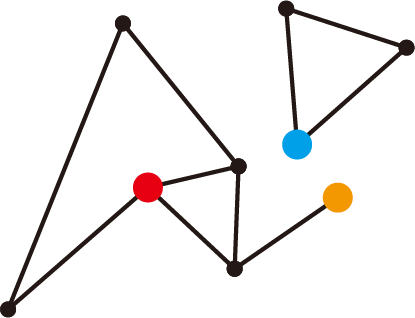
\includegraphics[width = 0.25\linewidth]{./images/connected_1.png}
\end{figure}

\begin{proposition} \label{connectivity}
    图 $ G = (n, m) $, 若存在一条 $ v_i $ 到 $ v_j $ 的道路, 当且仅当一定存在一条 $ v_i $ 到 $ v_j $ 的长度不大于 $ n - 1 $ 的道路.
\end{proposition}

\begin{proof}
    充分条件是不证自明的.

    对于必要条件, 若存在一条 $ v_i $ 到 $ v_j $ 的道路, 如果其长度大于 $ n - 1 $, 则其中必然存在重复的点. 如 $ v_1, v_2, \dots, v_i, \dots, v_j, \dots, v_k $, 其中 $ v_i = v_j $, 则可以删掉 $ v_i $ 到 $ v_j $ 的回路, 构造出一条更短的道路: $ v_1, \dots, v_i, v_{j + 1}, \dots, v_k $. 重复上面的过程, 当没有重复点的时候, 其长度必然不大于 $ n - 1 $.
\end{proof}

所以 $ G = (n, m) $ 中, $ u $ 和 $ v $ 是连通的充要条件可以等价地强化为存在一条 $ a $ 到 $ b $ 或 $ b $ 到 $ a $ 的长度不大于 $ n - 1 $ 的道路.

\begin{definition}[\text{连通分支}]
    设 $ G $ 为无向图, 则 $ G $ 的一个连通分支是 $ G $ 的一个子图 $ G' $, 且 $ G' $ 不是另一连通分支的子图. 换句话说, $ G $ 的连通分支是 $ G $ 的一个极大连通子图. 图 $ G $ 连通分支的个数记作为 $ \omega(G) $.
\end{definition}

\paragraph{例}
下图用红蓝橙三种颜色标注出了三个连通分支, 该图的连通分支数 $ \omega(G) = 3 $:
\begin{figure}[H]
    \centering
    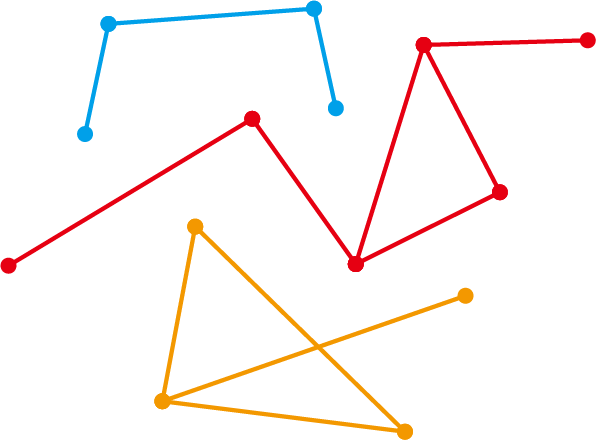
\includegraphics[width = 0.3\linewidth]{./images/branch.png}
\end{figure}



\subsection{连通度}
\begin{definition}[\text{点割集/割点}]
    设 $ G = (V, E) $ 为无向连通图, $ V' \subseteq V $. 若删去 $ V' $ 后, $ G - V' $ 不再连通, 则称 $ V' $ 为 $ G $ 的一个点割集. 若 $ V' $ 是单元素集, 则这个点 $ v $ 称为割点.
\end{definition}

\begin{definition}[\text{边割集/割边}]
    设 $ G = (V, E) $ 为无向连通图, $ E' \subseteq E $. 若删去 $ E' $ 后, $ G - E' $ 不再连通, 则称 $ E' $ 为 $ G $ 的一个边割集. 若 $ V' $ 是单元素集, 则这个边 $ e $ 称为割边或桥.
\end{definition}

\paragraph{例}
下图中, 删除蓝色的点, 原本的连通图变得不再连通, 所以这个点为一个割点. 删除红色的边, 图也变得不连通, 所以这条边为一条割边(或桥).
\begin{figure}[H]
    \centering
    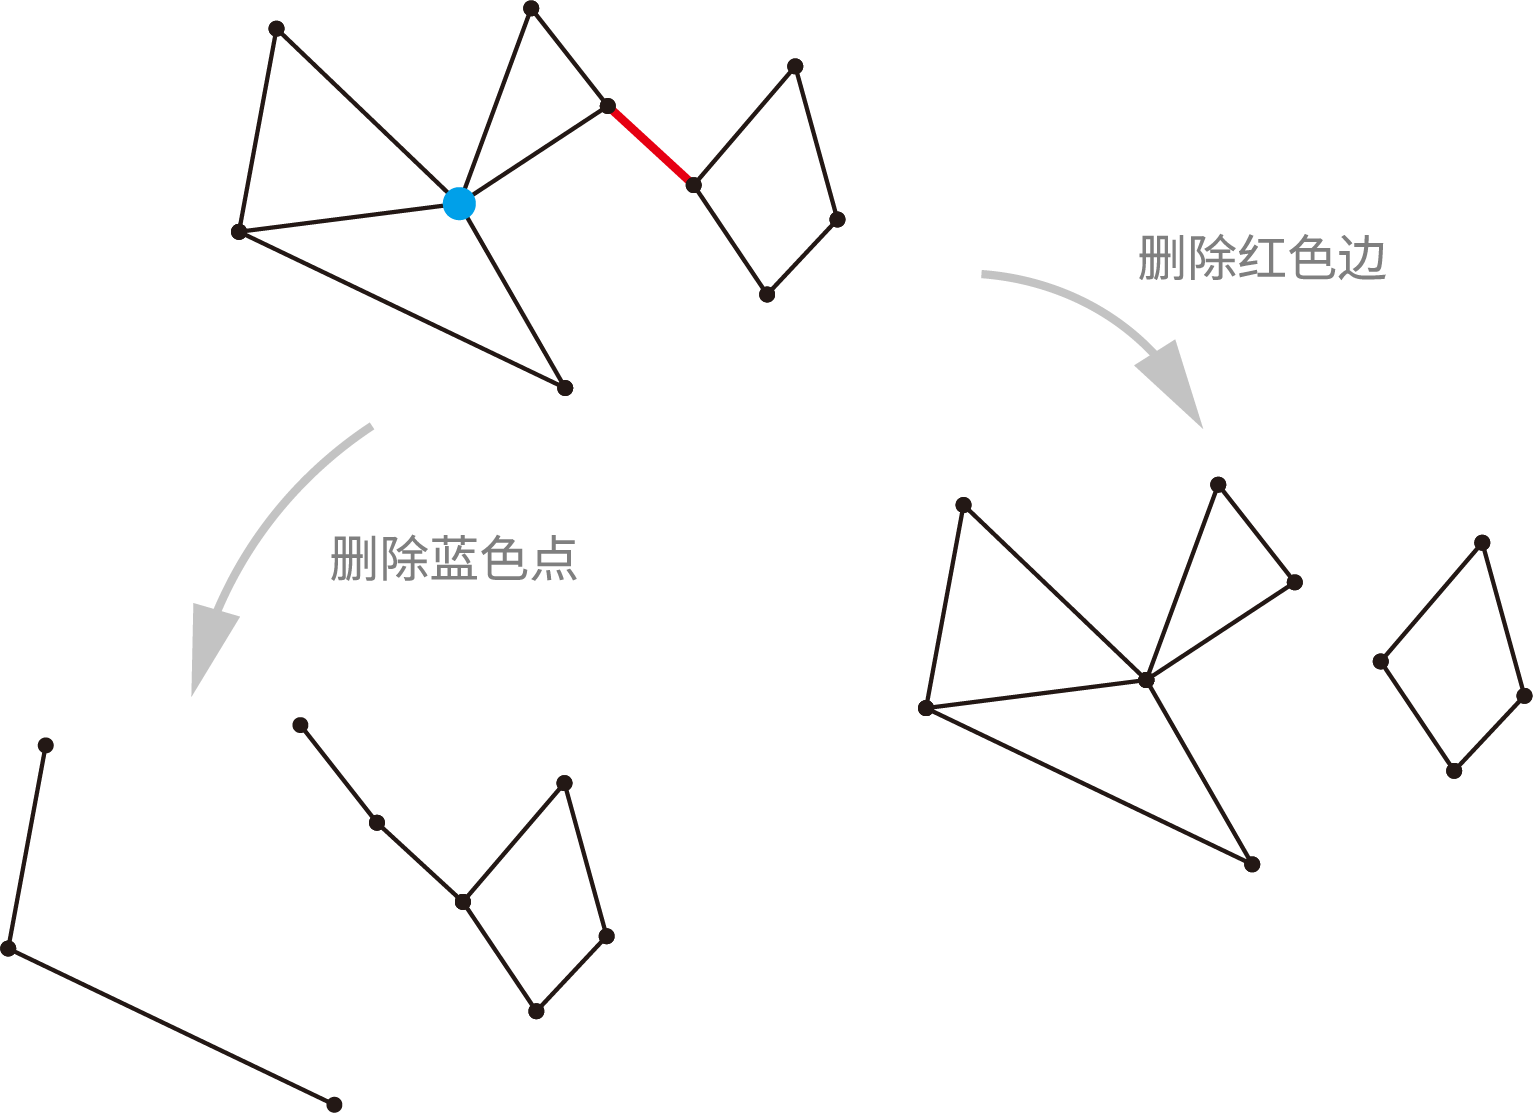
\includegraphics[width = 0.7\linewidth]{./images/bridge.png}
\end{figure}


\begin{definition}[\text{连通度}]
    设 $ G $ 的点割集族为 $ \set{V_1, V_2, \dots, V_n} $, 则定义点连通度(简称连通度)为:
    \[ \kappa(G) \coloneqq \min\set{|V_1|, |V_2|, \dots, |V_n|} \,,\]

    即最小的点割集基数. 同理可以定义边连通度 $ \lambda(G) $.
\end{definition}

换句话说, 点/边连通度描述了使图不再连通需要删除的最少的点/边的数量. 容易得到, 对于 $ n $ 个点 $ 0 \leqslant \kappa(G) \leqslant n - 1 $, $ 0 \leqslant \lambda(G) \leqslant n - 1 $. 而如果 $ G $ 本就是不连通的, 则定义 $ \kappa(G) = \lambda(G) = 0 $, 因为无需删点/边就能达到不连通. $ n $ 个顶点的图, 连通度不能为 $ n $, 因为删去所有顶点没有意义.

注意到一点, 对于完全图 $ K_n $, 无论删去多少点, 图总是连通的, 所以定义 $ K_n $ 的点连通度和边连通度 $ \kappa(K_n) = \lambda(K_n) = n - 1 $, 后面会说明, $ n $ 阶非完全图的最大连通度只能大到 $ n - 2 $, 所以剩下的 $ n - 1 $ 分配给完全图是很自然的.

综上所述, 可以通过给定点连通度, 图有两种情况:
\begin{itemize}
    \item 点连通度为 $ 0 $: $ G $ 不连通或 $ G $ 只有一个顶点 (即 $ K_1 $)
    \item 点连通度为 $ 1 $: $ G $ 最少删去 $ 1 $ 个顶点就不再连通, 或 $ G $ 为完全图 $ K_2 $
    \item 点连通度为 $ n $: $ G $ 最少删去 $ n $ 个顶点就不再连通, 或 $ G $ 为完全图 $ K_{n + 1} $
\end{itemize}

\paragraph{例}



\begin{proposition}
    无向图中, 下面三个命题等价:
    \begin{itemize}
        \item $ \kappa(G) = n - 1 $
        \item $ \lambda(G) = n - 1 $
        \item $ G $ 是完全图 $ K_n $
    \end{itemize}
    也就是说: 若 $ n $ 顶点图 $ G $ 不是完全图, 则 $ \kappa(G) \leqslant n - 2 $, $ \lambda(G) \leqslant n - 2 $.
\end{proposition}

\begin{proposition}
    设有无向图 $ G $, 其点连通度 $ \kappa(G) $, 边连通度 $ \lambda(G) $ 和最小点度 $ \delta(G) $ 存在不等关系:
    \[ \kappa(G) \leqslant \lambda(G) \leqslant \delta(G) \,.\] 
    当(且仅当? 待证)边割集中的边无公共端点时, $ \kappa(G) = \lambda(G) $.
\end{proposition}

\begin{proof}
    证明 $ \lambda(G) \leqslant \delta(G) $: 取度最小的点 $ v $, $ d(v) = \delta(G) $. 删除与 $ v $ 关联的所有边, 一定能够使图不连通. 删除了 $ \delta(G) $ 条边, 边连通图 $ \lambda(G) \leqslant \delta(G) $.

    证明 $ \kappa(G) \leqslant \lambda(G) $: 考虑最小的边割集 \[ \set{e_i \mid 1 \leqslant i \leqslant \lambda(G)} \,.\] 如果删除边割集中所有边关联的对应的两个端点之一, 则整个边割集中的边也都被删去, 图也就不连通. 当边割集中的边没有公共端点时, 删去每一条边的端点会导致不连通, 因而此时 $ \kappa(G) = \lambda(G) $; 而当边割集中的边存在公共端点时, 删去公共端点, 多条边被同时删去, 故此时需要删去的端点就少于边割集中边的数量, $ \kappa(G) < \lambda(G) $.
\end{proof}


\section{图的表示}
\subsection{邻接矩阵}
设 $ \ve A = (a_{ij})_{n \times n} $ 为图 $ G $ 的邻接矩阵. 矩阵的幂 $ \ve A^n = \ve A \ve A \cdots \ve A $ 里包含了 $ G $ 中长度为 $ n $ 的道路(不妨称其 $ 1- $道路)的信息.

\begin{remark}
    $ \ve A^n = \ve A \ve A \cdots \ve A $ 区别于 $ \ve A^{[n]} = \ve A \odot \ve A \odot \cdots \odot \ve A $.
\end{remark}

令 $ w_{ij}^{(k)} $ 表示 $ v_i $ 到 $ v_j $ 的长度为 $ k $ 的道路数目. 显然: $ w_{ij}^{(1)} = a_{ij} $. 考虑 $ \ve B = \ve A^2 $: 
\[ 
    b_{ij} = \sum_{\gamma = 1}^{n} a_{i\gamma} a_{\gamma j} = \sum_{\gamma = 1}^{n} w_{i \gamma}^{(1)} a_{\gamma j}^{(1)} \,.
\]
而对于每一个 $ \gamma \in [1..n] $, $ w_{i\gamma}^{(1)} $ 为 $ v_i $ 到 $ v_\gamma $ 的 $ 1- $道路数, $ w_{\gamma j}^{(1)} $ 为 $ v_{\gamma} $ 到 $ v_j $ 的 $ 1- $道路数, 那么从计数原理中的乘法公式中, 可以知道: $ w_{i \gamma}^{(1)} w_{\gamma j}^{(1)} $ 表示 $ v_i $ 到途经 $ v_{\gamma} $ 到达 $ v_j $ 的道路数, 且该道路长度为 $ 2 $.

那么 $ w_{i1}^{(1)} w_{1j}^{(1)} + w_{i2}^{(1)} w_{2j}^{(1)} + \dots + w_{in}^{(1)} w_{nj}^{(1)} $ 自然就得到 $ v_i $ 到 $ v_j $ 的 $ 2- $道路数.


\begin{proposition}
    若图 $ G $ 的邻接矩阵为 $ \ve A_{n \times n} $, 则 $\bigl( \ve A^k \bigr)_{ij} $ 表示 $ v_i $ 到 $ v_j $ 的长度为 $ k $ 的道路数. 换句话说, 令 $ \ve B = \ve A^k $, 则 $ b_{ij} = w_{ij}^{(k)} $.
\end{proposition}

\begin{proof}
    对 $ k $ 归纳. 当 $ k = 1 $ 时, $ b_{ij} = a_{ij} = w_{ij}^{(1)} $. 这是基础情形. 现归纳地假设当 $ \ve B = \ve A^k $ 时, $ b_{ij} = w_{ij}^{(k)} $. 证明当 $ \ve B = \ve A^{k + 1} $ 时, $ b_{ij} = w_{ij}^{(k + 1)} $.

    当 $ \ve B = \ve A^{k + 1} $ 时, 设 $ \ve C = \ve A^k $, 于是 $ \ve B = \ve C \ve A $:
    \[ 
        b_{ij} = \sum_{\gamma = 1}^{n} c_{i \gamma} a_{\gamma j} \,,
    \]
    而根据归纳假设和基础情形 $ c_{i \gamma} = w_{i \gamma}^{(k)} $, $ a_{i \gamma} = w_{i \gamma}^{(1)} $. 所以:
    \[ 
        b_{ij} = \sum_{\gamma = 1}^{n} w_{i \gamma}^{(k)} w_{\gamma j}^{(1)} \,.
    \]
    下面说明等式右侧就等于 $ w_{ij}^{(k + 1)} $. 下面为表述方便, 引入记号 $ \set[\big]{u \connect[k] v} $ 表示起点为 $ u $ 终点为 $ v $ 的长度为 $ k $ 的道路集合. 我们需要证明对于任意 $ 1 \leqslant \alpha < \beta \leqslant n $, 道路 $ \set[\big]{v_i \connect[k] v_\alpha \connect[1] v_j} $ 和 $ \set[\big]{v_i \connect[k] v_\beta \connect[1] v_j} $ 互斥, 这样同一条道路才不会被计算多次. 使用反证法, 假设存在一条 $ v_i \connect[k] v_\alpha \connect[1] v_j $ 和一条 $ v_i \connect[k] v_\beta \connect[1] v_j $ 相同, 记作 $ P $, 于是 $ v_\alpha $ 和 $ v_\beta $ 同在 $ P $ 上. 注意 $ v_\alpha \neq v_\beta $, 所以 $ v_\alpha $ 和 $ v_\beta $ 必然一前一后, 不失一般性地假设 $ P \colon v_i, \dots, v_\alpha, \dots, v_\beta, \dots, v_j $, 所以 $ d(v_i, v_\alpha) \neq d(v_i, v_\beta) $, 这与 $ d(v_i, v_\alpha) = d(v_i, v_\beta) = k $ 的假设矛盾.

    所以等式右侧 $ \sum\limits_{\gamma = 1}^{n} w_{i \gamma}^{(k)} w_{\gamma j}^{(1)} = w_{ij}^{(k + 1)} $, 这便完成了归纳.
\end{proof}

所以我们得到了两点不连通的条件:
\begin{corollary}
    若图 $ G = (n, m) $ 的邻接矩阵为 $ \ve A $. 若对任意 $ 1 \leqslant k \leqslant n - 1 $, 都有:
    \[ 
        \bigl( \ve A^k \bigr)_{ij} = 0 \,,
    \]
    则 $ v_i $ 和 $ v_j $ 不连通. 其中: $ \bigl( \ve A^k \bigr)_{ij} $ 表示 $ \ve A^k $ 的 $ i $ 行 $ j $ 列元素.
\end{corollary}

\begin{proof}
    条件说明 $ v_i $ 和 $ v_j $ 间不存在长度小于 $ n - 1 $ 的道路, 由命题 \ref{connectivity}, $ v_i $ 和 $ v_j $ 之间不存在道路.
\end{proof}


\subsection{可达性矩阵与关系矩阵}
图的可达性矩阵中, 若 $ v_i $ 和 $ v_j $ 连通则对应元素为 $ 1 $, 这一概念与关系矩阵高度关联. 事实上, 图 $ G $ 的可达性矩阵就是 $ G $ 表示的关系 $ R $ 的传递闭包的矩阵表示.





\end{document}